\documentclass[a4paper, 12pt]{article}

\usepackage{cmap}
\usepackage[OT1]{fontenc}
\usepackage[utf8]{inputenc}
%\usepackage{mathtext}
%\usepackage{amsmath}
\usepackage[russian]{babel}
\usepackage{amsmath}
\usepackage{amsfonts}
\usepackage{amssymb}
\usepackage{graphicx}
%\usepackage[bookmarks=true, pdfpagemode=UseNone]{hyperref}
\usepackage{indentfirst}
\usepackage{listings}
%\usepackage{multicol}
%\usepackage{misccorr}
%\usepackage{longtable}
%\usepackage{flafter}
\usepackage{float}
%\usepackage{color}
%\usepackage{nccfloats}
%\usepackage{tabularx}
%\usepackage{graphicx}
%\usepackage[babel=true,protrusion=true,expansion=true]{microtype}
%\usepackage[left=1.8cm, right=1cm, top=1cm, bottom=1cm, bindingoffset=0cm]{geometry}

%\pagestyle{empty}

\author{Алексюк А.О., Мурашко Д.С.}
\title{Линейная фильтрация}
\lstset{inputencoding=utf8, extendedchars=\true, keepspaces = true, language=Matlab}

\begin{document}
\maketitle
\tableofcontents
\pagebreak

\section{Цель работы}
Изучить воздействие ФНЧ на тестовый сигнал с шумом.

\section{Постановка задачи}
Сгенерировать гармонический сигнал с шумом и синтезировать ФНЧ. Получить сигнал во временной и частотной областях до и после фильтрации. Сделать выводы о воздействии ФНЧ на спектр сигнала.

\section{Ход работы}
Линейный фильтр - динамическая система, применяющая некий линейный оператор ко входному сигналу для выделения или подавления определенных частот сигнала и других функций по обработке входного сигнала.
Фильтр Баттерворта - один из типов электронных фильтров. Фильтры этого класса отличаются от других методом проектирования. Фильтр Баттерворта проектируется так, чтобы его амплитудно-частотная характеристика
была максимально гладкой на частотах полосы пропускания.
В командном окне Matlab сгенерируем гармонический сигнал без шума
и с шумом, а также спектры сигнала с шумом и без шума. 

\subsection{Код Matlab}
\begin{lstlisting}
x = 0:0.01:4*pi;
f=100*(0:255)/512;
figure
noise=rand(size(x));
y = sin(2*pi*x);
y_noisy = y+0.3*noise;
%Построение сигнала без шума:
plot(x(1:200),y(1:200))
grid
%синтез ФНЧ Баттерворта
[B,A] = butter(16,0.99);
B=B./sum(B);
A=A./sum(A);
%обработка сигнала ФНЧ
figure
y_filtered = conv(y_noisy,[B,A]);
%Построение сигнала с шумом:
plot(x(1:200),y_filtered(1:200))
grid
figure
%Построение спектра сигнала с шумом
noisy_spectrum = fft(y_noisy,512);
norm_noisy_spectrum = noisy_spectrum.*conj(noisy_spectrum)/512;
%Построение нормирова спектра сигнала с шумом:
plot(f,norm_noisy_spectrum(1:256))
axis([0 max(f) 0 2])
grid
figure
%Спектр сигнала без шума
spectrum = fft(y_filtered,512);
norm_filtered_spectrum=spectrum.*conj(spectrum)/512;
%Построение нормированого спектра сигнала без шума:
plot(f,norm_filtered_spectrum(1:256))
axis([0 max(f) 0 2])
grid

\end{lstlisting}

\begin{figure}[H]
   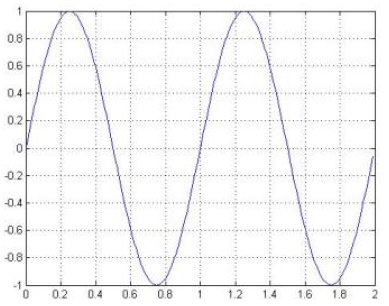
\includegraphics[scale=0.7]{lab6/1.png}
   \caption{Сигнал без шума}
\end{figure}

\begin{figure}[H]
   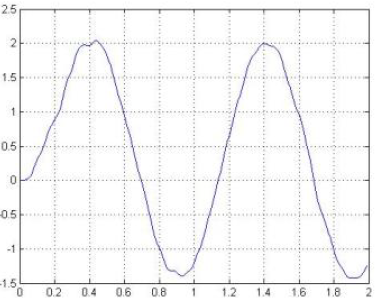
\includegraphics[scale=0.7]{lab6/2.png}
   \caption{Сигнал с шумом}
\end{figure}

\begin{figure}[H]
   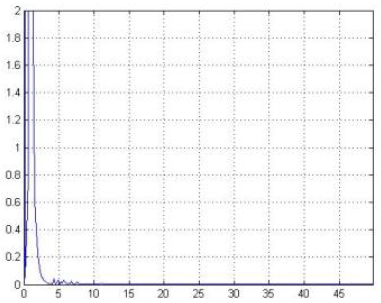
\includegraphics[scale=0.7]{lab6/3.png}
   \caption{Спектр сигнала без шума}
\end{figure}

\begin{figure}[H]
   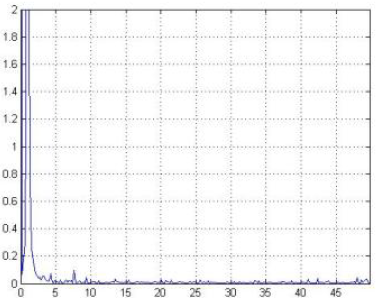
\includegraphics[scale=0.7]{lab6/4.png}
   \caption{Спектр сигнала с шумом}
\end{figure}

\subsection{Simulink}
Для создания модели в Simulink
используем блок Discrete FIR Filter раздела Discrete главной библиотеки и
блок Digital Filter design из Signal Processing Blockset/Filtering/Filter Designs.

\begin{figure}[H]
   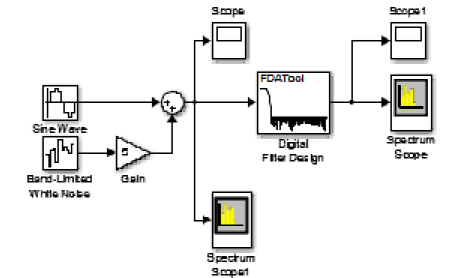
\includegraphics[scale=0.7]{lab6/5.png}
   \caption{Схема модели}
\end{figure}

\begin{figure}[H]
   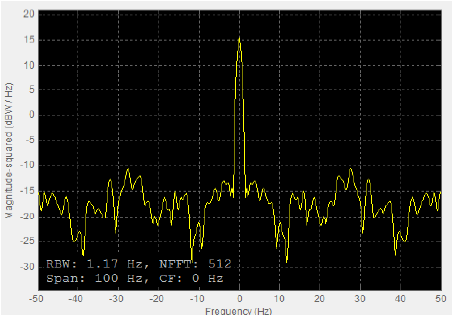
\includegraphics[scale=0.7]{lab6/6.png}
   \caption{Спектр до фильтрации}
\end{figure}

\begin{figure}[H]
   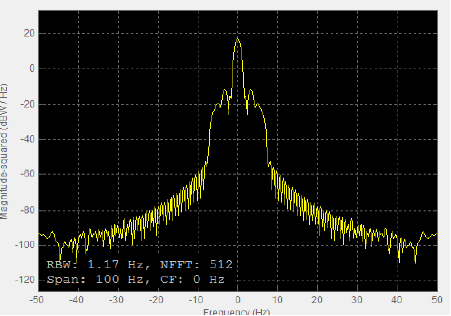
\includegraphics[scale=0.7]{lab6/7.png}
   \caption{Спектр после фильтрации}
\end{figure}
\begin{figure}[H]
   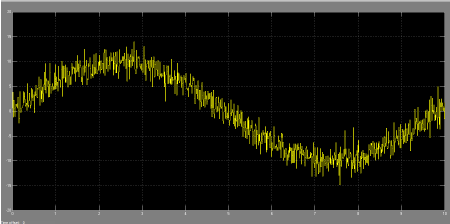
\includegraphics[scale=0.7]{lab6/8.png}
   \caption{Спектр сигнала без шума}
\end{figure}

\begin{figure}[H]
   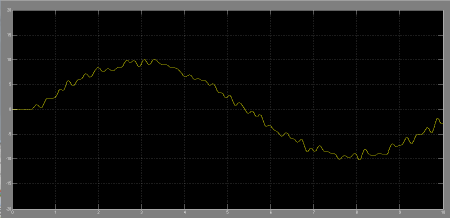
\includegraphics[scale=0.7]{lab6/9.png}
   \caption{Спектр сигнала с шумом}
\end{figure}

\section{Вывод}

Фильтр нижних частот - один из видов аналоговых или электронных фильтров, эффективно пропускающий частотный спектр сигнала ниже некоторой частоты (частоты среза), и уменьшающий (подавляющий) частоты сигнала выше этой частоты. Степень подавления каждой частоты зависит от
вида фильтра. В лабораторной работе мы произвели неполное удаление шума линейным фильтром. Для его полного удаления нам необходим идеальный фильтр (с прямоугольным окном). Линейная фильтрация не устраняет
полностью шум, т.к. для полного удаления необходим идеальный фильтр
с прямоугольным окном, которого на практике не существует. Так же, т.к. линейный фильтр подавляет все сигналы, находящиеся в его полосе задержания и не изменяет сигналы из полосы пропускания, то он не может
удалить шум, который попал в его полосу пропускания. Соответственно
удалить весь шум он не в силах.
	

\end{document}